%\documentclass[12pt]{article}
 %\documentclass[letterpaper,floatfix,citeautoscript,aip,jcp]{revtex4-1}
 %\documentclass[letterpaper,floatfix,citeautoscript,showkeys]{revtex4-1}
 %\documentclass[twocolumn,letterpaper,floatfix,citeautoscript,jcp]{revtex4-1}
 %\documentclass[twocolumn,letterpaper,floatfix,citeautoscript,aip,jcp]{revtex4-1}
 \documentclass[journal=jced,manuscript=article]{achemso}
 \setkeys{acs}{maxauthors=30,etalmode=truncate,articletitle=true}
 %%%%%%%%%%%%%%%%%%%%%%%%%%%%%%%%%%%%%%%%%%%%%%%%%%%%%%%%%%%%%%%%%%%%%
 %% Place any additional packages needed here.  Only include packages
 %% which are essential, to avoid problems later.
 %%%%%%%%%%%%%%%%%%%%%%%%%%%%%%%%%%%%%%%%%%%%%%%%%%%%%%%%%%%%%%%%%%%%%
 \usepackage{chemformula} % Formula subscripts using \ch{}
 \usepackage[T1]{fontenc} % Use modern font encodings
 
 %%%%%%%%%%%%%%%%%%%%%%%%%%%%%%%%%%%%%%%%%%%%%%%%%%%%%%%%%%%%%%%%%%%%%
 %% If issues arise when submitting your manuscript, you may want to
 %% un-comment the next line.  This provides information on the
 %% version of every file you have used.
 %%%%%%%%%%%%%%%%%%%%%%%%%%%%%%%%%%%%%%%%%%%%%%%%%%%%%%%%%%%%%%%%%%%%%
 %%\listfiles
 
 %%%%%%%%%%%%%%%%%%%%%%%%%%%%%%%%%%%%%%%%%%%%%%%%%%%%%%%%%%%%%%%%%%%%%
 %% Place any additional macros here.  Please use \newcommand* where
 %% possible, and avoid layout-changing macros (which are not used
 %% when typesetting).
 %%%%%%%%%%%%%%%%%%%%%%%%%%%%%%%%%%%%%%%%%%%%%%%%%%%%%%%%%%%%%%%%%%%%%
% \newcommand*\mycommand[1]{\texttt{\emph{#1}}}

\usepackage{fullpage}
\usepackage{amsfonts}
\usepackage{graphicx}
\usepackage{float}
\usepackage{amsmath}
\usepackage{chemfig}
\usepackage{indentfirst}
\usepackage{longtable}
\usepackage{array}
\usepackage{cellspace}
\usepackage{palatino}
%\usepackage{breqn}
\usepackage{amssymb}
\usepackage{verbatim}
\usepackage[hidelinks,colorlinks=false,citecolor=black,linkcolor=black]{hyperref}
\usepackage{siunitx}
\usepackage{xr}

\makeatletter
\newcommand*{\addFileDependency}[1]{% argument=file name and extension
	\typeout{(#1)}
	\@addtofilelist{#1}
	\IfFileExists{#1}{}{\typeout{No file #1.}}
}
\makeatother

\newcommand*{\myexternaldocument}[1]{%
	\externaldocument{#1}%
	\addFileDependency{#1.tex}%
	\addFileDependency{#1.aux}%
}

\myexternaldocument{JCED_FOMMS_supporting_information}

\SectionNumbersOn

% The figures are in a figures/ subdirectory.
\graphicspath{{figures/}}

%\bibliographystyle{apsrevlong}
%\bibliographystyle{apsrev}
\bibliographystyle{unsrt}

% italicized boldface for math (e.g. vectors)
\newcommand{\bfv}[1]{{\mbox{\boldmath{$#1$}}}}
% non-italicized boldface for math (e.g. matrices)
\newcommand{\bfm}[1]{{\bf #1}}          

%\newcommand{\bfm}[1]{{\mbox{\boldmath{$#1$}}}}
%\newcommand{\bfm}[1]{{\bf #1}}
\newcommand{\expect}[1]{\left \langle #1 \right \rangle} % <.> for denoting expectations over realizations of an experiment or thermal averages

\newcommand{\var}[1]{{\mathrm var}{(#1)}}
\newcommand{\x}{\bfv{x}}
\newcommand{\y}{\bfv{y}}
\newcommand{\f}{\bfv{f}}

\newcommand{\hatf}{\hat{f}}

\newcommand{\bTheta}{\bfm{\Theta}}
\newcommand{\btheta}{\bfm{\theta}}
\newcommand{\bhatf}{\bfm{\hat{f}}}
\newcommand{\Cov}[1] {\mathrm{cov}\left( #1 \right)}
\newcommand{\T}{\mathrm{T}}                                % T used in matrix transpose

\newcommand\blfootnote[1]{%
	\begingroup
	\renewcommand\thefootnote{}\footnote{#1}%
	\addtocounter{footnote}{-1}%
	\endgroup
}

\author{Richard A. Messerly}
\email{richard.messerly@nist.gov}
\affiliation{Thermodynamics Research Center, National Institute of Standards and Technology, Boulder, Colorado, 80305, United States}

\author{Mohammad S. Barhaghi}
\affiliation{Department of Chemical Engineering and Materials Science, Wayne State University, Detroit, Michigan 48202, United States}

\author{Jeffrey J. Potoff}
\affiliation{Department of Chemical Engineering and Materials Science, Wayne State University, Detroit, Michigan 48202, United States}

\author{Michael R. Shirts}
\affiliation{Department of Chemical and Biological Engineering, University of Colorado, Boulder, Colorado, 80309, United States}

%%%%%%%%%%%%%%%%%%%%%%%%%%%%%%%%%%%%%%%%%%%%%%%%%%%%%%%%%%%%%%%%%%%%%
%% The document title should be given as usual. Some journals require
%% a running title from the author: this should be supplied as an
%% optional argument to \title.
%%%%%%%%%%%%%%%%%%%%%%%%%%%%%%%%%%%%%%%%%%%%%%%%%%%%%%%%%%%%%%%%%%%%%
%\title{Multistate Bennett Acceptance Ratio replaces histogram reweighting for vapor-liquid coexistence calculations}
%\title{Multistate Bennett Acceptance Ratio to enable rapid force field parameterization}
%\title{Multistate Bennett Acceptance Ratio as a substitute for histogram reweighting when optimizing non-bonded parameters}
%\title{Multistate reweighting provides a better alternative to histogram reweighting for coexistance calculations}
\title{Multistate histogram-free reweighting for vapor-liquid coexistence calculations of non-simulated force field parameters}
%\title{Estimating vapor-liquid coexistence properties with histogram-free reweighting}

%%%%%%%%%%%%%%%%%%%%%%%%%%%%%%%%%%%%%%%%%%%%%%%%%%%%%%%%%%%%%%%%%%%%%
%% Some journals require a list of abbreviations or keywords to be
%% supplied. These should be set up here, and will be printed after
%% the title and author information, if needed.
%%%%%%%%%%%%%%%%%%%%%%%%%%%%%%%%%%%%%%%%%%%%%%%%%%%%%%%%%%%%%%%%%%%%%
%\abbreviations{IR,NMR,UV}
\keywords{MBAR}

%%%%%%%%%%%%%%%%%%%%%%%%%%%%%%%%%%%%%%%%%%%%%%%%%%%%%%%%%%%%%%%%%%%%%
%% The manuscript does not need to include \maketitle, which is
%% executed automatically.
%%%%%%%%%%%%%%%%%%%%%%%%%%%%%%%%%%%%%%%%%%%%%%%%%%%%%%%%%%%%%%%%%%%%%
\begin{document}
	
	%%%%%%%%%%%%%%%%%%%%%%%%%%%%%%%%%%%%%%%%%%%%%%%%%%%%%%%%%%%%%%%%%%%%%
	%% The "tocentry" environment can be used to create an entry for the
	%% graphical table of contents. It is given here as some journals
	%% require that it is printed as part of the abstract page. It will
	%% be automatically moved as appropriate.
	%%%%%%%%%%%%%%%%%%%%%%%%%%%%%%%%%%%%%%%%%%%%%%%%%%%%%%%%%%%%%%%%%%%%%
%	\begin{tocentry}
%	\end{tocentry}

\blfootnote{Contribution of NIST, an agency of the United States government; not subject to copyright in the United States.}

\section*{Abstract}

\section{Introduction}

A key advancement in molecular simulation is the ability to accurately and efficiently estimate vapor-liquid coexistence properties, i.e., saturated liquid density $(\rho_{\rm liq}^{\rm sat})$, saturated vapor density $(\rho_{\rm vap}^{\rm sat})$, saturated vapor pressures $(P_{\rm vap}^{\rm sat})$, and enthalpy of vaporization $(\Delta H_{\rm v})$. The accuracy of coexistence estimates depends on the underlying molecular model (a.k.a., force field, potential model, or Hamiltonian) while the computational efficiency depends primarily on the simulation methods. Due to the abundance of experimental vapor-liquid coexistence data and the sensitivity of such properties to both short- and long-range non-bonded interactions, numerous force fields have been parameterized using $\rho_{\rm liq}^{\rm sat}$, $P_{\rm vap}^{\rm sat}$, and $\Delta H_{\rm v}$. Although the development of accurate force fields has been greatly enabled by the improved efficiency of simulation methods, parameterization of non-bonded interactions with vapor-liquid coexistence calculations remains an arduous and time-consuming task \cite{TraPPE,TAMie,Mie}.

Several methods exist for computing vapor-liquid coexistence properties, e.g., Gibbs Ensemble Monte Carlo (GEMC), two phase molecular dynamics (2$\phi$MD), isothermal-isochoric integration (ITIC), and Grand Canonical Monte Carlo coupled with histogram reweighting (GCMC-HR). Advantages and disadvantages exist for each method. For example, GEMC and GCMC require insertion moves that are computationally inefficient for complex molecular structures with high density liquid phases. Several advanced simulation techniques are available to overcome this challenge \cite{ConBias}, which has enabled GEMC and GCMC-HR to be the primary methods of choice for vapor-liquid coexistence calculations.

Some clear advantages and disadvantages exist for GCMC-HR compared with GEMC. For example, one advantage of GCMC-HR is the higher precision \cite{GEMC_GCMC}. Furthermore, coexistence properties can be computed at temperatures that are not simulated directly. However, GEMC is arguably more straightforward in that simulations are performed only at the desired saturation temperatures $(T^{\rm sat})$. By contrast, GCMC-HR requires a series of GCMC simulations for a single $T^{\rm sat}$. This set includes a near-critical simulation that ``bridges'' the vapor and liquid phases. Obtaining the appropriate chemical potential $(\mu)$ for this bridge simulation is a cumbersome and, typically, iterative process (although more advanced methods exist to obtain a good initial estimate for $\mu$ \cite{Hemmen2015}).

Another disadvantage of GCMC-HR compared to GEMC is that GCMC-HR requires more post-processing (i.e., histogram reweighting), while simple block averaging is typically sufficient for GEMC. Histogram reweighting (and more generally, configuration reweighting) is an important tool in many fields of molecular simulation. In fact, it has long since been known that it is possible to estimate properties for state ``j'' by reweighting configurations that were sampled with state ``i.'' \cite{McDonald1967,Card1970,Wood1968,Pana2000} For example, umbrella sampling simulations are often processed using the weighted histogram analysis method (WHAM) to compute free energy differences between states. A popular alternative to WHAM is the Multistate Bennett Acceptance Ratio (MBAR) \cite{chodera:jctc:2007,shirts-chodera:jcp:2008:mbar}, which is readily available in the \textit{pymbar} package.

In this study, we substitute HR with MBAR for the GCMC-HR approach of computing vapor-liquid coexistence properties. Section \ref{sec: MBAR} demonstrates that MBAR and HR are mathematically equivalent (in the limit of zero bin width) while Section \ref{sec: Results} shows that they are also numerically equivalent (to within statistical uncertainties). Note that, as Boulougouris et al. demonstrate how to combine HR with GEMC (GEMC-HR) to estimate saturation properties at non-simulated temperatures \cite{Boulougouris2010}, MBAR could alternatively be applied to GEMC simulations.

%and example scripts are included as Supporting Information to promote future implementation.  

%In this study, we utilize an alternative to histogram reweighting, namely, the Multistate Bennett Acceptance Ratio (MBAR) . MBAR is readily available in the \textit{pymbar} package and example scripts are included as Supporting Information to promote future implementation. Section \ref{sec: MBAR} demonstrates that MBAR and HR are mathematically equivalent (in the limit of zero bin width) while Section \ref{sec: Results} shows that they are also numerically equivalent (to within statistical uncertainties). Note that Boulougouris et al. combine HR with GEMC (GEMC-HR) to estimate saturation properties at non-simulated temperatures \cite{Boulougouris2010}. Therefore, although we apply MBAR to GCMC simulations, the approach can also be applied to GEMC simulations.

%In this study, we utilize the Multistate Bennett Acceptance Ratio (MBAR) Grand Canonical Monte Carlo (GCMC-MBAR) as a substitute for GCMC-HR. We demonstrate that MBAR and HR are mathematically equivalent (in the limit of zero bin width) as well as practically equivalent (to within statistical uncertainties). Note that Boulougouris et al. demonstrate how HR can be applied to GEMC output (GEMC-HR) to estimate saturation properties at non-simulated temperatures \cite{Boulougouris2010}. Therefore, although we apply MBAR to GCMC simulations, the approach can also be applied to GEMC simulations.
%
%
%
%Although GEMC appears to be slightly more popular amongst simulation practitioners, this study utilizes the GCMC approach. GCMC-HR has been shown to

%In this study we demonstrate how the Multistate Bennett Acceptance Ratio is mathematically equivalent to histogram reweighting 
%%% Old version
%Although GCMC-HR has a higher precision than GEMC, GEMC remains a more popular method amongst simulation practitioners. There are at least two potential reasons why GEMC has grown in popularity relative to GCMC-HR. First, GEMC is more straightforward in that, GEMC simulations are performed directly at the desired saturation temperature $(T^{\rm sat})$. By contrast, GCMC-HR requires a series of GCMC simulations for a single $T^{\rm sat}$ (although this is also an advantage of GCMC-HR as estimates can be obtained at any $T^{\rm sat}$ value without additional simulations). This set includes a near-critical simulation that ``bridges'' the vapor and liquid phases. Obtaining an initial guess for the chemical potential $(\mu)$ of this bridge simulation is a cumbersome and, typically, iterative process, although more advanced methods do exist to obtain a good initial estimate for $\mu$ (e.g., Hemmen et al. \cite{Hemmen2015}). 
%
%A likely second reason for increased popularity of GEMC is that GCMC-HR requires a great deal of post-processing (i.e., histogram reweighting), while simple block averaging is typically sufficient for GEMC. In this study, we introduce an alternative to histogram reweighting, namely, the Multistate Bennett Acceptance Ratio (MBAR) \cite{chodera:jctc:2007,shirts-chodera:jcp:2008:mbar}. MBAR is readily available in the \textit{pymbar} package and example scripts are included as Supporting Information to promote future implementation.
%
%Histogram reweighting (and more generally, configuration reweighting) is an important tool in many fields of molecular simulation. In fact, it has long since been known that it is possible to estimate properties for state ``j'' by reweighting configurations that were sampled with state ``i.'' \cite{McDonald1967,Card1970,Wood1968,Pana2000} For example, umbrella sampling simulations are often processed using the weighted histogram analysis method (WHAM) to compute free energy differences between states. In addition, Boulougouris et al. demonstrated how histogram reweighting can be applied to GEMC output to estimate saturation properties at non-simulated temperatures (analogous to GCMC-HR) \cite{Boulougouris2010}.
%
%Although the development of accurate force fields has been greatly enabled by the efficiency of the aforementioned simulation methods (e.g., GEMC, GCMC-HR), parameterization of non-bonded interactions with vapor-liquid coexistence calculations remains an arduous and time-consuming task \cite{TraPPE,TAMie,Mie}. MBAR-GCMC not overly serves as a substitute for MBAR-HR, but MBAR can also be used to estimate properties for non-simulated parameter sets. For example, recently, Messerly et al. demonstrated how MBAR coupled with ITIC (MBAR-ITIC) enables rapid force field parameterization by estimating coexistence properties for non-simulated parameter sets \cite{Postdoc_1,Postdoc_2}. 

%
%Although histogram reweighting requires additional analysis steps, the benefits of histogram reweighting are clear. For example

%Although histogram reweighting approaches are common in some fields of molecular simulation, e.g., WHAM is commonly used for computing free energies, most open-source Monte Carlo codes do not include a HR tool and, thus, in-house post-processing codes abound. In this study, we introduce an alternative to histogram reweighting, namely, the Multistate Bennett Acceptance Ratio (MBAR). MBAR is readily available in the \textit{pymbar} package and example scripts are included as Supporting Information to promote future implementation.

%, with a near-critical simulation that ``bridges'' the vapor and liquid phases.

%For example, the exponential-6 model of Errington and Panagiotoupoulos
%The method outlined in this study is similar in spirit to the ``Hamiltonian scaling'' (HS) approach utilized with GEMC (BLANK) and GCMC-HR (BLANK).

%A closely related method to histogram reweighting, and one that is similar in spirit to the method outlined in the present study, is ``Hamiltonian scaling'' (HS). Despite Hamiltonian scaling Grand Canonical Monte Carlo (HS-GCMC) proving to be a powerful tool to obtain coexistence curves for multiple force fields from a single set of simulations, it has yet to gain widespread popularity. This is likely due to the added complexity of the algorithm, where the prescribed $\mu$ and $T$ change during the coarse of the GCMC simulation, depending on which Hamiltonian (force field) is being sampled. Furthermore, the post-processing requires a slightly more complicated form of histogram reweighting. Also, HS requires a decision be made \textit{a priori} regarding which Hamiltonians are to be tested. By contrast, MBAR does not require any modification of the simulation procedure, the post-processing is essentially unchanged, and the Hamiltonians need not be selected prior to the simulations.
 
Substituting the standard HR approach with MBAR is not the primary purpose of this study. Rather, we demonstrate how GCMC-MBAR can also estimate coexistence properties for non-simulated parameter sets, which can greatly accelerate force field parameterization. In a similar study, Messerly et al. demonstrate how to combine MBAR with ITIC (MBAR-ITIC) to optimize Mie $\lambda$-6 (generalized Lennard-Jones) potentials \cite{Postdoc_1,Postdoc_2}. For MBAR-ITIC, a series of $NVT$ simulations along an isotherm and isochores are performed with a ``reference'' force field $(\theta_{\rm ref})$. MBAR computes the internal energy $(U)$ and pressure $(P)$ (or compressibility factor, $Z$) for each $T-\rho$ state point with a non-simulated (``rerun'') force field $(\theta_{\rm rr})$. ITIC then converts the $U$ and $P$ values into vapor-liquid coexistence properties \cite{Mostafa_Diss,Mostafa2018}.

%, where $U$ and $P$ are estimated by performing $NVT$ simulations and reweighting the configurations with MBAR.

% at numerous temperatures and densities, \cite{Mostafa_Diss,Mostafa2018} these values are estimated by performing $NVT$ simulations and reweighting the configurations with MBAR.

The results from Messerly et al. demonstrate that MBAR-ITIC is most reliable in the local domain, i.e., for parameter sets near the ``reference'' parameter set from which configurations are sampled \cite{Postdoc_1}. Furthermore, MBAR-ITIC performs best for changes in the non-bonded well-depth parameter $(\epsilon)$ while it performs significantly worse for large changes in the non-bonded size and repulsive parameters $(\sigma$ and $\lambda$, respectively$)$. This is typically referred to as poor ``overlap'' and can be quantified by the ``number of effective samples'' $(N_{\rm eff})$. Poor overlap (low $N_{\rm eff}$) is especially problematic for ITIC as a large number of snapshots is needed to obtain precise estimates of $P$ in the liquid phase, which are essential to obtain reasonable values of $\rho_{\rm liq}^{\rm sat}$.

%MBAR not only serves as a substitute for histogram reweighting in the standard GCMC-HR approach, but GCMC-MBAR can also be used to estimate coexistence properties for non-simulated parameter sets, which can greatly accelerate force field parameterization. In a similar study, Messerly et al. demonstrate how to combine MBAR with ITIC (MBAR-ITIC) to optimize Mie $\lambda$-6 (generalized Lennard-Jones) potentials \cite{Postdoc_1,Postdoc_2}. Since ITIC requires the internal energy $(U)$ and pressure $(P)$ (or compressibility factor, $Z$) at numerous temperatures and densities, \cite{Mostafa_Diss,Mostafa2018} these values are estimated by performing $NVT$ simulations and reweighting the configurations with MBAR. 

%The results from Messerly et al. demonstrate that MBAR-ITIC is most reliable in the local domain, i.e., for parameter sets near the ``reference'' parameter set from which configurations are sampled \cite{Postdoc_1}. Furthermore, MBAR-ITIC performs best for changes in the non-bonded well-depth parameter $(\epsilon)$ while it performs significantly worse for large changes in the non-bonded size and repulsive parameters $(\sigma$ and $\lambda$, respectively$)$. This is typically referred to as poor ``overlap.''

Our hypothesis is that GCMC-MBAR should have better overlap over the non-bonded parameter space than what was observed for MBAR-ITIC. There are two main reasons for this hypothesis/aspiration. First, the fluctuating densities of GCMC simulations, as opposed to the fixed density $NVT$ simulations, accommodate a wider range of configurations and energies. Second, ITIC requires accurate calculations of $U$ and $P$ in the vapor phase, which necessitate larger box sizes (and, thereby, more molecules) than those typically utilized with GCMC. By utilizing fewer molecules, GCMC simulations experience larger energy fluctuations (on a percent basis) which improves the overlap between states. We also hypothesize that the impact of poor overlap is less severe compared to ITIC, where poor overlap leads to sporadic coexistence estimates.  

%  require a large number of snapshots ITIC requires precise estimates of $P$ in the liquid phase, which necessitates a large number of of snapshots for

%configurations. $(NVT)$ does not sample from a wide range of energies  leads to large energy differences for small changes in $\sigma$ and $\lambda$. The fluctuating densities of GCMC simulations should accommodate greater changes in short-range interactions. 

Note that the method outlined in this study is similar in spirit to ``Hamiltonian scaling'' (HS), which has been applied to both GEMC and GCMC simulations. The HS approach samples from multiple force fields (Hamiltonians) in a single simulation according to a weighted sampling probability. Vapor-liquid coexistence curves for each force field are estimated post-simulation by reweighting the configurations accordingly. For the Grand Canonical Monte Carlo implementation of Hamiltonian scaling (HS-GCMC), $\mu$ and $T$ are not stationary during the simulation, rather the current value of $\mu$ and $T$ depends on which force field is being sampled. Despite HS-GCMC proving to be a powerful tool to optimize force field parameters \cite{Errington1998,Exp6,Errington1999,Pana2000}, it has yet to gain widespread popularity. This is likely due to the added complexity of both the simulation protocol and the histogram post-processing. Also, HS requires that a decision be made \textit{a priori} regarding which force fields are to be tested. By contrast, MBAR does not require any modification of the simulation procedure, the post-processing is essentially unchanged, and the non-bonded parameter sets need not be selected prior to the simulations.

Recently, Weidler and Gross proposed ``individualized,'' i.e., compound-specific, parameter sets for compounds which contain large amounts of experimental data \cite{Weidler2018}. To avoid overfitting, a one-dimensional optimization is employed which scales $\epsilon$ for all united-atom sites while not adjusting $\sigma$ or $\lambda$. MBAR is ideally suited for this ``$\epsilon$-scaling'' approach for at least two reasons. First, as mentioned previously, MBAR is most reliable when extrapolating in $\epsilon$ rather than $\sigma$ and/or $\lambda$. Second, the rate-limiting step for MBAR is recomputing the configurational energies for a different force field. Furthermore, storing millions of configuration ``snapshots'' is highly memory intensive. While basis functions (see Section \ref{sec: Basis functions}) alleviate the additional computational cost and reduce the memory load, $\epsilon$-scaling does not require storing/recomputing configurations or basis functions. Instead, the energies for each snapshot are simply multiplied by the $\epsilon$-scaling parameter.  

%   Despite HS-GCMC proving to be a powerful tool to obtain coexistence curves for multiple force fields from a single set of simulations, it has yet to gain widespread popularity. This is likely due to the added complexity of the algorithm, where the prescribed $\mu$ and $T$ change during the coarse of the GCMC simulation, depending on which Hamiltonian (force field) is being sampled. Furthermore, the post-processing requires a slightly more complicated form of histogram reweighting. Also, HS requires a decision be made \textit{a priori} regarding which Hamiltonians are to be tested. By contrast, MBAR does not require any modification of the simulation procedure, the post-processing is essentially unchanged, and the Hamiltonians need not be selected prior to the simulations.

%The results from Messerly et al. demonstrated that MBAR is accurate over a wide range of $\epsilon$ (the Lennard-Jones well-depth parameter) values but less reliable for large changes in $\sigma$ (the Lennard-Jones size parameter) and $\lambda$ (the Mie $\lambda$-6 repulsive parameter, i.e., for Lennard-Jones 12-6 $\lambda = 12$). MBAR is most reliable in the local parameter space relative to the reference parameter set from which configurations are sampled.

%Some fundamental limitations exist for the MBAR-ITIC approach. First, ITIC is ill-suited for near-critical saturation properties, i.e., ITIC is not recommended for $T^{\rm sat} > 0.85 T_{\rm c}$ ($T_{\rm c}$ is the critical temperature). Second, ITIC requires a temperature correlation for the virial coefficients of the force field. Third, the poor extrapolation of MBAR with changes in $\sigma$ and $\lambda$.

The outline for this study is the following. Section \ref{sec: Methods} provides details regarding the force fields, simulation set-up, and post-simulation analysis with MBAR. Section \ref{sec: Results} provides a comparison of GCMC-MBAR and GCMC-HR as well as various applications of GCMC-MBAR for force field parameterization. Section \ref{sec: Discussion} discusses some limitations and provides recommendations for future work. Section \ref{sec: Conclusions} presents the primary conclusions.

% for of GCMC-MBAR  validates that GCMC-MBAR yields indistinguishable results from GCMC-HR, applies GCMC-MBAR to $\epsilon$-scaling, and . We demonstrate how
%
%\begin{enumerate}
%	\item Accurate and efficient computation of vapor-liquid coexistence is an important but challenging task for molecular simulation
%	\item Reweighting simulation outputs between different states is a well-known and powerful tool, e.g., histogram reweighting of GCMC results
%	\item Force field parameterization with VLE data is an arduous and time-consuming task
%	\item Hamiltonian scaling (histogram reweighting for multiple force fields) allows for estimating VLE properties of multiple force fields from single set of simulations
%	\item Messerly et al. demonstrated how MBAR can be combined with ITIC to predict VLE properties. Several  Weakness of ITIC is need large systems, which is not ideal for MBAR
%	\item Gross demonstrated benefits of $\epsilon$-scaling for ``individualized'', i.e., compound-specific parameter sets
%	\item In this study, we demonstrate that:
%	\begin{enumerate}
%		\item MBAR yields indistinguishable results from histogram reweighting (HR)
%		\item Scaling epsilon is straightforward by scaling U with MBAR
%		\item MBAR can estimate VLE properties for multiple force fields simultaneously
%		\item Basis functions allow for rapid computation of VLE for non-simulated Mie parameter sets
%	\end{enumerate}
%\end{enumerate}

\section{Methods} \label{sec: Methods}

\subsection{Force fields} \label{sec: Force fields}

    The force fields utilized in this study are Transferable Potentials for Phase Equilibria (TraPPE-UA, also referred to simply as TraPPE \cite{TraPPE,Martin1999,TraPPEUA2}), Potoff \cite{Mie,Potoff_branched}, and Nath, Escobedo, and de Pablo revised (NERD). Each force field adopts a united-atom (UA) representation, where non-polar hydrogens are not modeled explicitly. The non-bonded potential is of the generalized Lennard-Jones (Mie $\lambda$-6) form. 
    
    The bond lengths for the TraPPE, Potoff, and NERD force fields are 0.154 nm for all compounds studied. The same angle and dihedral potentials are used for each force field. Angular bending interactions are evaluated using a harmonic potential:
    \begin{equation}
    u^{\rm bend} = \frac{k_\theta}{2} \left(\theta-\theta_0\right)^2
    \end{equation}
    where $u^{\rm bend}$ is the bending energy, $\theta$ is the instantaneous bond angle, $\theta_0$ is the equilibrium bond angle (see Table \ref{tab:angles}), and $k_\theta$ is the harmonic force constant with $k_\theta/k_{\rm B} = 62500$ K/rad$^2$ for all bonding angles, where $k_{\rm B}$ is the Boltzmann constant. 
    
    \begin{table}[h!]
    	\caption{Equilibrium bond angles $(\theta_0)$ \cite{Martin1999}. CH$_i$ and CH$_j$ represent CH$_3$, CH$_2$, CH, or C sites.} \label{tab:angles}
    	\begin{center}
    		\begin{tabular}{|c|c|}
    			\hline
    			Bending sites & $\theta_0$ (degrees) \\ \hline
    			CH$_i$-CH$_2$-CH$_j$ & 114.0 \\ 
    			CH$_i$-CH-CH$_j$ & 112.0 \\ 
    			CH$_i$-C-CH$_j$ & 109.5 \\  
    			\hline
    		\end{tabular}
    	\end{center} 
    \end{table}
    
    Dihedral torsional interactions are determined using a cosine series:
    \begin{equation}
    u^{\rm tors} = c_0 + c_1 [1+\cos{\phi}] + c_2 [1-\cos{2\phi}] + c_3 [1+\cos{3\phi}]
    \end{equation}
    where $u^{\rm tors}$ is the torsional energy, $\phi$ is the dihedral angle and $c_n$ are the Fourier constants listed in Table \ref{tab:torsions}.
    
    \begin{table}[h!]
    	\caption{Fourier constants $(c_n/k_{\rm B})$ in units of K \cite{Martin1999}. CH$_i$ and CH$_j$ represent CH$_3$, CH$_2$, CH, or C sites.} \label{tab:torsions}
    	\begin{center}
    		\begin{tabular}{|c|c|c|c|c|}
    			\hline
    			Torsion sites & $c_0/k_{\rm B}$ & $c_1/k_{\rm B}$ & $c_2/k_{\rm B}$ & $c_3/k_{\rm B}$ \\ \hline
    			CH$_i$-CH$_2$-CH$_2$-CH$_j$ & 0.0 & 355.03 & -68.19 & 791.32 \\ 
    			CH$_i$-CH$_2$-CH-CH$_j$ & -251.06 & 428.73 & -111.85 & 441.27 \\
    			CH$_i$-CH$_2$-C-CH$_j$ & 0.0 & 0.0 & 0.0 & 461.29 \\
    			CH$_i$-CH-CH-CH$_j$ & -251.06 & 428.73 & -111.85 & 441.27 \\
    			\hline
    		\end{tabular}
    	\end{center} 
    \end{table}
    
    Non-bonded interactions between sites located in two different molecules or separated by more than three bonds within the same molecule are calculated using a Mie $\lambda$-6 potential (of which the Lennard-Jones, LJ, 12-6 is a subclass):
    \begin{equation} \label{eq:Mie}
    u^{\rm nb}(\epsilon,\sigma,\lambda;r) = \left(\frac{\lambda}{\lambda - 6}\right)\left(\frac{\lambda}{6}\right)^{\frac{6}{\lambda - 6}} \epsilon \left[\left(\frac{\sigma}{r}\right)^{\lambda} - \left(\frac{\sigma}{r}\right)^6\right]
    \end{equation} 
    where $u^{\rm nb}$ is the van der Waals interaction, $\sigma$ is the distance $(r)$ where $u^{\rm nb} = 0$, $-\epsilon$ is the energy of the potential at the minimum $\left(\text{i.e., }u^{\rm nb} = -\epsilon \text{ and } \frac{\partial u^{\rm nb}}{\partial r} = 0 \text{ for } r=r_{\rm min} \right)$, and $\lambda$ is the repulsive exponent. 
    
    The non-bonded Mie $\lambda$-6 force field parameters for TraPPE, Potoff, and NERD are provided in Table \ref{tab:nonbonded params}. Potoff reports a ``generalized'' and ``short/long'' (S/L) CH and C parameter set. The ``short'' and ``long'' parameters are implemented when the number of carbons in the backbone is $\le 4$ and $> 4$, respectively. Also note that the NERD force field has several different parameter sets for CH$_3$ sites.
    
%%% Old format
%    \begin{table}[h!]
%    	\caption{Non-bonded (intermolecular) parameters for TraPPE \cite{TraPPE,Martin1999}, Potoff \cite{Mie,Potoff_branched}, and NERD \cite{NERD}. The ``short/long'' Potoff CH and C parameters are included in parentheses.} \label{tab:nonbonded params}
%    	\begin{center}
%    		\begin{tabular}{|c|c|c|c|c|c|c|}
%    			\hline
%    			United-atom & $\epsilon/k_{\rm B}$ (K) & $\sigma$ (nm) & $\lambda$ & $\epsilon/k_{\rm B}$ (K) & $\sigma$ (nm) & $\lambda$ \\ \hline
%    			\multicolumn{1}{|c}{} & \multicolumn{3}{|c}{TraPPE} & \multicolumn{3}{|c|}{Potoff (S/L)}  \\ \hline
%    			CH$_3$ & 98 (134.5)  & 0.375 (0.352) & 12 & 121.25 & 0.3783 & 16  \\ 
%    			CH$_2$ & 46 & 0.395 & 12 & 61 & 0.399 & 16 \\ 
%    			CH & 10 & 0.468 & 12 & 15 (15/14) & 0.46 (0.47/0.47) & 16\\
%    			C & 0.5 & 0.640 & 12 & 1.2 (1.45/1.2) & 0.61 (0.61/0.62) & 16\\
%    			\hline
%    			\multicolumn{1}{|c}{} & \multicolumn{3}{|c}{NERD} & \multicolumn{3}{|c|}{} \\ \hline
%    			CH$_3$ & 104.00  & 0.3910 & 12 & -- & -- & --\\ 
%                CH$_3$ (2-methylpropane) & 78.23  & 0.3880 & 12 & -- & -- & --\\ 
%                CH$_3$ (2,2-dimethylpropane) & 74.50  & 0.3910 & 12 & -- & -- & --\\ 
%                CH$_3$ & 104.00  & 0.3910 & 12 & -- & -- & --\\ 
%    			CH$_2$ & 45.80 & 0.3930 & 12 & -- & -- & -- \\ 
%    			CH & 39.70 & 0.3850 & 12 &  -- & -- & --\\
%    			C & 17.00 & 0.3910 & 12 & -- & -- & --\\
%    			\hline
%    		\end{tabular}
%    	\end{center} 
%    \end{table}

    \begin{table}[h!]
		\caption{Non-bonded (intermolecular) parameters for TraPPE \cite{TraPPE,Martin1999}, Potoff \cite{Mie,Potoff_branched}, and NERD \cite{NERD}.} \label{tab:nonbonded params}
		\begin{center}
			\begin{tabular}{|c|c|c|c|}
				\hline
				United-atom & $\epsilon/k_{\rm B}$ (K) & $\sigma$ (nm) & $\lambda$ \\ \hline
				\multicolumn{1}{|c}{} & \multicolumn{3}{|c|}{TraPPE} \\ \hline
				CH$_3$ & 98 (134.5)  & 0.375 (0.352) & 12 \\ 
				CH$_2$ & 46 & 0.395 & 12\\ 
				CH & 10 & 0.468 & 12 \\
				C & 0.5 & 0.640 & 12 \\
				\hline
				\multicolumn{1}{|c}{} & \multicolumn{3}{|c|}{Potoff} \\ \hline
				CH$_3$ & 121.25 & 0.3783 & 16  \\ 
				CH$_2$ & 61 & 0.399 & 16 \\ 
				CH, gen. & 15 & 0.46 & 16\\
				C, gen. & 1.2 & 0.61 & 16\\
				CH, short & 15 & 0.47 & 16\\
				C, short & 1.45 & 0.61 & 16\\
				CH, long & 14 & 0.47 & 16\\
				C, long & 1.2 & 0.62 & 16\\
				\hline
				\multicolumn{1}{|c}{} & \multicolumn{3}{|c|}{NERD} \\ \hline
				CH$_3$ & 104.00  & 0.3910 & 12\\ 
				CH$_3$ (2-methylpropane) & 78.23  & 0.3880 & 12\\ 
				CH$_3$ (2,2-dimethylpropane) & 74.50  & 0.3910 & 12 \\ 
%				CH$_3$ & 104.00  & 0.3910 & 12\\ 
				CH$_2$ & 45.80 & 0.3930 & 12 \\ 
				CH & 39.70 & 0.3850 & 12\\
				C & 17.00 & 0.3910 & 12 \\
				\hline
			\end{tabular}
		\end{center} 
	\end{table}
    
    Non-bonded parameters between two different site types (i.e., cross-interactions) are determined using Lorentz-Berthelot combining rules \cite{Allen1987} for $\epsilon$ and $\sigma$ and an arithmetic mean for the repulsive exponent $\lambda$ (as recommended in Reference \citenum{Mie}):
    \begin{equation} \label{eq:Lorentz-Berthelot_eps}
    \epsilon_{ij} = \sqrt{\epsilon_{ii} \epsilon_{jj}}
    \end{equation}
    \begin{equation} \label{eq:Lorentz-Berthelot_sig}
    \sigma_{ij} = \frac{\sigma_{ii} + \sigma_{jj}}{2}
    \end{equation}
    \begin{equation} \label{eq:Lorentz-Berthelot_lam}
    \lambda_{ij} = \frac{\lambda_{ii} + \lambda_{jj}}{2}
    \end{equation}
    where the $ij$ subscript refers to cross-interactions and the subscripts $ii$ and $jj$ refer to same-site interactions. 
    
%\begin{enumerate}
%	\item Simulations are performed for united-atom generalized Lennard-Jones (a.k.a., Mie $\lambda$-6) force fields
%	\item We investigate the TraPPE, Potoff-generalized, Potoff (S/L), and NERD force fields 
%	\item Details of force fields
%\end{enumerate}

\subsection{Simulation set-up} \label{sec: Simulation set-up}

The majority of results presented in Section \ref{sec: Results} are obtained by reprocessing simulation output that were analyzed in previous studies utilizing histogram reweighting \cite{Potoff_branched,Barhaghi2017}. New simulation results are provided for \textit{n}-hexane, 2-methylpropane, 2,2-dimethylpropane, 2,2,4-trimethylhexane, 2,3-dimethylbutane, 2,3,4-trimethylpentane, 2,2,3,3-tetramethylbutane, and cyclohexane. All simulations are performed using GPU optimized Monte Carlo (GOMC) with Grand Canonical Monte Carlo (GCMC), where the chemical potential ($\mu$), volume $(V)$, and temperature $(T)$ are constant. 

A series of nine simulations are performed, two in the vapor phase, six in the liquid phase, and one near critical which acts as the ``bridge'' between the vapor and liquid phases. A low-density (less than twenty molecules) initial configuration is utilized for the vapor phase simulations, while the bridge and liquid phase simulations are initialized with a high-density (around 200 molecules) configuration. The system volume is the same for each simulation, but varies somewhat between compounds. The prescribed chemical potentials and temperatures for the branched alkanes are the same as those utilized in Mick et al. \cite{Potoff_branched}. The $\mu-T$ values for \textit{n}-hexane and cyclohexane are determined in this study. All state points are reported in Supporting Information. 

The equilibration stage for each GCMC simulation consists of $2 \times 10^7$ Monte Carlo steps (MCS). The production stage is $4 \times 10^7$ MCS for vapor simulations and $2.5 \times 10^7$ MCS for the liquid and ``bridge'' simulations. Snapshots (i.e., number of molecules, internal energy, and optionally the xyz coordinates) are stored every 200 MCS to reduce the correlation between sequential configurations. Thus, the total number of snapshots $(N_{\rm snaps})$ is $2 \times 10^5$ for vapor simulations and $1.25 \times 10^5$ for liquid and ``bridge'' simulations. The type of Monte Carlo move implemented for each step is selected randomly with a 20\%, 10\%, and 70\% probability of performing a displacement, rotation, and particle swap move, respectively. The move probabilities are slightly different for cyclohexane, namely, 30\%, 10\%, 40\%, and 20\% for displacement, rotation, particle swap, and crank-shaft moves, respectively.  

%, where a Monte Carlo cycle is defined as $N$ individual Monte Carlo steps

Four different applications for MBAR are demonstrated in this study, where slightly different types of simulation output are required. First, we demonstrate how MBAR yields consistent results to those previously reported using histogram reweighting. The standard simulation output is used in this application, namely, a 2x$N_{\rm snaps}$ array containing the number of molecules and the internal energy for all $N_{\rm snaps}$ snapshots. Second, we demonstrate how these same data can be used with MBAR to predict VLE properties when performing $\epsilon$-scaling. Third, we investigate how well MBAR can predict VLE for force field ``j'' from sampled states of force field ``i.'' In this case, a 3x$N_{\rm snaps}$ array is required, where the additional column is the internal energy computed with force field ``j'' for the configurations sampled with force field ``i.'' Fourth, we demonstrate how storing basis functions is a computationally efficient method for predicting VLE for multiple force fields that are unknown at runtime.   

%\begin{enumerate}
%	\item Simulations performed by Mick et al. are reanalyzed using MBAR
%	\item Additional simulations are performed in GCMC ensemble using GPU optimized Monte Carlo (GOMC)
%	\item Simulation specifications, i.e., box size, number of steps, type of moves, etc.
%	\item State points (chemical potentials and temperatures) simulated are same as those utilized in Mick et al.
%\end{enumerate}

\subsection{Multistate Bennett Acceptance Ratio} \label{sec: MBAR}

The GCMC approach for estimating phase coexistence requires significant post-processing. Before demonstrating how we implement MBAR for this purpose, we review the traditional histogram reweighting approach. We also discuss the steps of this procedure that are the same for both HR and MBAR. We refer the interested reader to the literature for derivations and more detailed discussion of the GCMC-HR equations (cf. \citenum{Pana2000}).


%\begin{eqnarray} \label{HR prob}
%Pr(N,U) = \frac{\Omega (N,V,U) \exp (-\beta U + \beta \mu N)}{\Xi (\mu, V, \beta)}
%\end{eqnarray}

MRSHIRTS: I would like the MBAR and histogram reweighting equations to be consistent with each other in the limit of zero bin-width and a single reference force field. Here is how HR is presented in the literature, verbatim:

The probability of observing $N$ particles with internal energy $U$ for a given chemical potential $(\mu)$ and inverse temperature $(\beta \equiv \frac{1}{k_{\rm B}T}$ where $k_{\rm B}$ is the Boltzmann constant) is
%%% This is how the equation is presented in Pana2000, but I want to have similar terms between MBAR and HR
\begin{eqnarray} \label{eq: HR prob lit}
p(N,E;\mu,\beta) = \frac{\sum_{i=1}^{R} f_i(N,E)  \exp(-\beta E + \beta \mu N)}{\sum_{i=1}^{R} K_i \exp(-\beta_i U + \beta_i \mu_i N - C_i)}
\end{eqnarray}
where $f_i(N,E)$ is the probability of occurrence $N$ particles in the simulation cell with total configurational energy in the vicinity of $E$, $K_i$ is the total number of observations $(K_i = \sum_{N,E} f_i(N,E))$ for run $i$. The constants $C_i$ (also known as ``weights'') are obtained by iteration from the relationship
\begin{eqnarray} \label{eq: Weights lit}
\exp (C_i) = \sum_{E} \sum_{N} p(N,E;\mu_i,\beta_i)
\end{eqnarray}
Given an initial guess for the set of weights $C_i$, Equations \ref{eq: HR prob lit} and \ref{eq: Weights lit} can be iterated until convergence. The ensemble average for a given observable is
\begin{eqnarray}
\langle O \rangle_{\mu,\beta} = \sum_{E} \sum_{N} p(N,E;\mu,\beta) \times O
\end{eqnarray}
The pressure of a system can be obtained from the following expression. If the conditions for run 1 are $(\mu_1, V, \beta_1) and for run 2 (\mu_2, V, \beta_2)$, then
\begin{eqnarray} \label{eq: press lit}
C_2 - C_1 = \ln \frac{\Xi (\mu_2,V,\beta_2)}{\Xi (\mu_1,V,\beta_1)} = \beta_2 P_2 V - \beta_1 P_1 V
\end{eqnarray}
where $P$ is the pressure, since $\ln \Xi = \beta P V$. Equation \ref{eq: press lit} can be used to obtain the absolute value of the pressure for one of the two runs, provided that the absolute pressure can be estimated for the other run. Typically, this is done by performing simulations for low-density states for which the system follows the ideal gas equation of state, $P V = N k_{\rm B} T$.
 
%\begin{eqnarray} \label{HR prob}
%Pr(N,U|\mu,\beta) = \frac{\sum_{i=1}^{R} Pr_i(N,U)  \exp(-\beta U + \beta \mu N)}{\sum_{i=1}^{R} K_i \exp(-\beta_i U + \beta_i \mu_i N - C_i)}
%\end{eqnarray}

MRSHIRTS: Here is how I reported the MBAR equations in our first publication:

With MBAR the expectation $\langle O(\theta) \rangle$ for force field $(\theta)$ of any given observable $(O)$ can be expressed as:
\begin{eqnarray} \label{MBAR O theta}
\langle O(\theta)\rangle = \sum_{n=1}^{N} O(\x_{n};\theta) W_{n}(\theta)
\end{eqnarray}
where $\x_n$ are configurations sampled from one or more reference force fields $(\theta_{\rm ref})$, % is a set of samples collected from one or more previous simulations,
$O(\x_{n};\theta)$ is the observable value using force field 
$\theta$ with configurations $\x_n$, and $W_{n}(\theta)$ is the weight of the $n^{th}$
configuration using force field $\theta$, calculated by using:
\begin{eqnarray} \label{MBAR weights theta}
W_{n}(\theta) = \frac{\exp[\hat{f}(\theta)-u(\x_{n};\theta)]}{\sum\limits_{k=1}^K N_k \, \exp[\hat{f}(\theta_{\rm ref,k}) - u(\x_{n};\theta_{\rm ref,k})]}
\end{eqnarray}
where the reduced free energies $(\hat f(\theta))$ are calculated with:
\begin{eqnarray} \label{MBAR free energy theta}
\hat f(\theta) &=& - \ln \sum_{n=1}^{N^{\rm tot}_{\rm snaps}}
\frac{\exp[-u(\x_{n};\theta)]}{\sum\limits_{k=1}^K N_k \, \exp[\hat{f}(\theta_{\rm ref,k}) - u(\x_{n};\theta_{\rm ref,k})]} \label{equation:estimator-of-free-energies}
\end{eqnarray}
where $K$ is the number of reference force fields, $N^{\rm tot}_{\rm snaps} = \sum_k N_k$ is the total number of snapshots for all $K$ reference force fields, $N_k$ are the total number of snapshots from the $k^{th}$ reference force field, $\theta_{\rm ref,k}$ is the $k^{th}$ reference (i.e. simulated) force field, and $u(\x_{n};\theta)$ is the reduced potential energy evaluated with $\theta$ for configuration $\x_n$. For the grand canonical ensemble, $u(\x_{n};\theta) = \beta U(\x_n;\theta) - \beta \mu N$, where $\beta = \frac{1}{k_{\rm B}T}$ and $k_{\rm B}$ is the Boltzmann constant. 

Note that $\hat f(\theta_{\rm ref,k})$ is required to evaluate the denominator of Equations \ref{MBAR weights theta}-\ref{MBAR free energy theta}. The values for $\hat f(\theta_{\rm ref,k})$ are obtained by solving a system of $K$ equations for self-consistency. Specifically, an initial guess for $\hat f(\theta_{\rm ref,k})$ is used to evaluate Equation \ref{MBAR free energy theta} with $\theta=\theta_{\rm ref,k}$ to obtain updated values of $\hat f(\theta_{\rm ref,k})$. This process is repeated until the values for $\hat f(\theta_{\rm ref,k})$ converge to within a desired tolerance. Although solving the MBAR system of equations for self-consistency may require several iterations, fortunately, once this process has been performed $\hat f(\theta)$ (for an arbitrary $\theta$) is evaluated without further iteration.

The performance of MBAR depends strongly on good phase space overlap, meaning that the configurations sampled by the reference force field(s) must represent a significant portion of the ``true'' configurations that the non-simulated force field would sample \cite{naden:jctc:2016}. If the configurational overlap is small the MBAR estimates are likely dominated by a few configurations, which are likely not representative of the ensemble that would be generated by direct simulation of force field $\theta$. The amount of overlap can be quantified by the number of effective samples $(N_{\rm eff})$ \cite{Dybeck2016}, using Kish's formula:
\begin{eqnarray} \label{Neff}
N_{\rm eff} = \frac{\left(\sum_n W_n\right)^2}{\sum_n W_n^2}
\end{eqnarray}
which reduces to $N_{\rm eff} = (\sum_n W_n^2)^{-1}$ when the weights are
normalized. This has the property that when the weights are equal,
$N_{\rm eff} = N$, when all but one weight is negligible, $N_{\rm eff} \approx
1$, and behaves appropriately for intermediate cases. 
In the case of poor overlap $(N_{\rm eff} \approx 1)$, the predicted values of MBAR will demonstrate a strong bias and the uncertainties will likely be underestimated by the MBAR covariance matrix. 

\begin{enumerate}
	\item Traditionally, histogram reweighting (HR) has been applied with GCMC to calculate vapor-liquid coexistence properties
	\item Present histogram reweighting equations
	\item Discuss how to compute phase equilibria by equating pressures
	\item Discuss how to compute heat of vaporization
	\item In this study, we demonstrate how to compute VLE using MBAR-GCMC
	\item Procedure is identical to that utilized for HR but using the MBAR equations
	\item Present MBAR equations
	\item MBAR for $\theta = \theta_{\rm ref}$ is mathematically equivalent to histogram reweighting in the limit of zero bin width
	\item MBAR-GCMC allows for prediction of multiple force fields from single simulation without modifying force fields mid-simulation (i.e., Hamiltonian scaling approach)
	\item MBAR uncertainties are computed using bootstrap resampling
\end{enumerate}

\subsection{Basis functions} \label{sec: Basis functions}

\begin{enumerate}
	\item When applying MBAR to different parameter sets, $\theta \neq \theta_{\rm ref}$, it is necessary to recompute energies
	\item Basis functions accelerate the recompute energy step by storing the repulsive and attractive contributions that can be scaled by $\epsilon$ and $\sigma$
	\item Basis functions are computed from GOMC using the recompute feature for different $\epsilon$ and $\sigma$ and solving system of equations
\end{enumerate}

\section{Results} \label{sec: Results}

Section \ref{sec: MBAR} demonstrated that MBAR and HR are mathematically equivalent in the limit of zero bin width and when $\theta = \theta_{\rm ref}$. Figure \ref{fig:comparison MBAR HR} provides numerical validation that GCMC-MBAR and GCMC-HR yield indistinguishable vapor-liquid coexistence properties. Note that the median percent deviation is approximately zero and that the largest deviations are within a few percent. The percent deviations shown in Figure \ref{fig:comparison MBAR HR} are averaged over the 31 branched alkanes studied by Mick et al. and the 9 alkynes studied by Barhaghi et al. The GCMC-HR values were not recomputed in this study but were taken from the literature \cite{Potoff_branched,Barhaghi2017}. The GCMC-MBAR values were computed using the same raw simulation data as Mick et al. and Barhaghi et al. The only difference being that a single replicate was used to compute GCMC-MBAR values, whereas GCMC-HR used data from all five replicates. 

	\begin{figure}[htb!]
		\centering
		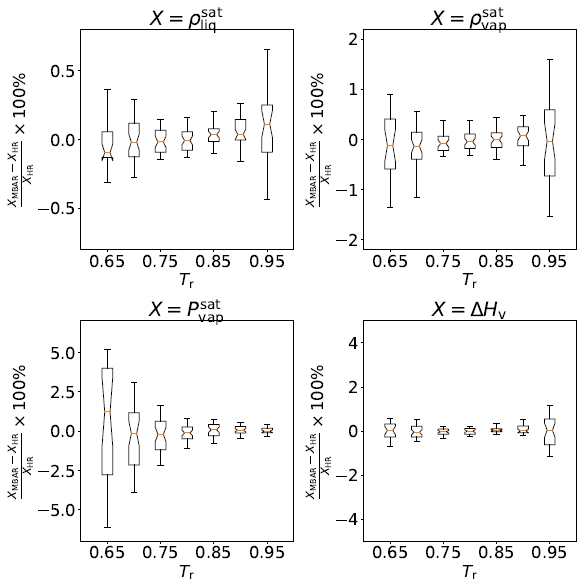
\includegraphics[width=6.4in]{Comparison_MBAR_HR_boxplot_CI.png}
		\caption{Percent deviations between coexistence properties computed using histogram reweighting (HR) and Multistate Bennett Acceptance Ratio (MBAR). Top-left, top-right, bottom-left, and bottom-right panels correspond to saturated liquid density, saturated vapor density, saturated vapor pressure, and enthalpy of vaporization, respectively. Boxes depict the first and third quartiles while whiskers represent the range that contains 95\% of the data.}
		\label{fig:comparison MBAR HR}
	\end{figure}

%(a), (b), (c), and (d)

Because it is not possible to visualize a parameter space of greater than two dimensions,   

These figures demonstrate the reliability of MBAR when multiple parameters are varied simultaneously. For example, all three non-bonded parameters ($\epsilon$, $\sigma$, and $\lambda$) for all four united-atom types (CH$_3$, CH$_2$, CH, and C) are different between the TraPPE and Potoff-gen force fields (see Figure \ref{fig:refFF_to_rrFF_lam12to16}). The TraPPE and NERD $\epsilon$ and $\sigma$ values are different for all four united-atom types while $\lambda = 12$ for both force fields. The Potoff-gen and Potoff-SL force fields only differ in the $\epsilon$ and/or $\sigma$ values for the CH and C sites. Specifically, the 2-methylpropane parameters are identical except for $\sigma_{\rm CH}$, the 2,2-dimethylpropane parameters are the same except for $\epsilon_{\rm C}$, and three parameters are different for 2,2,4-trimethylpentane ($\epsilon_{\rm CH}$, $\sigma_{\rm CH}$, and $\sigma_{\rm C}$). However, the difference in $\epsilon$ and $\sigma$ values is significantly smaller than that between TraPPE and NERD. 

Figures \ref{fig:refFF_to_rrFF_lam_constant} and \ref{fig:refFF_to_rrFF_lam12to16} compare the GCMC-MBAR predicted values for $\theta_{\rm rr} \neq \theta_{\rm ref}$ to those for $\theta_{\rm rr} = \theta_{\rm ref}$. Figure \ref{fig:refFF_to_rrFF_lam_constant} contains $\lambda_{rm rr} = \lambda_{\rm ref}$ while Figure \ref{fig:refFF_to_rrFF_lam12to16} corresponds to $\lambda_{rm rr} \neq \lambda_{\rm ref}$. Overall, MBAR is  The poor estimates of $\rho_{\rm liq}^{\rm sat}$ in Figure \ref{fig:refFF_to_rrFF_lam12to16} demonstrate that the repulsive exponent $(\lambda)$ greatly impacts the configurational overlap in the liquid phase.

	\begin{figure}[htb!]
		\centering
		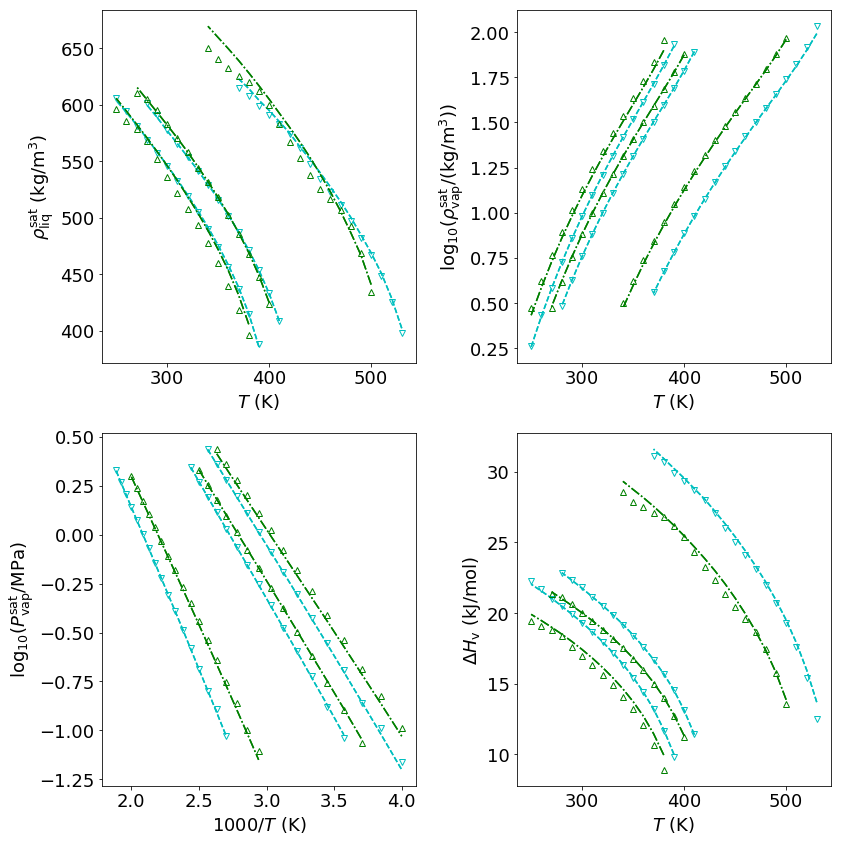
\includegraphics[width=6.4in]{refFF_to_rrFF_lam_constant.png}
		\caption{}
		\label{fig:refFF_to_rrFF_lam_constant}
	\end{figure}

	\begin{figure}[htb!]
		\centering
		\includegraphics[width=6.4in]{refFF_to_rrFF_lam12to16.png}
		\caption{}
		\label{fig:refFF_to_rrFF_lam12to16}
	\end{figure}


\begin{enumerate}
	\item We validate that MBAR and HR are indistinguishable by re-analyzing the simulation results of Mick et al. and Barhaghi et al. utilizing MBAR
	%	\begin{enumerate}
	%		\item Evaluate all of the compounds that Mohammad has U and N values for (branched alkanes and alkynes) and which have good experimental data
	%		\item Compare MBAR results with either Potoff's or my own HR results (might be better to use my own for self consistency)
	%	\end{enumerate}
	%    \item Validation of the basis function approach
	\item Epsilon scaling for all the compounds that Mohammad has U and N values for (branched alkanes and alkynes) and which have good experimental data
	\item We estimate Potoff generalized and NERD VLE from TraPPE simulations, Potoff S/L from Potoff generalized, and TraPPE from Potoff generalized
	\item For $\lambda_{\rm ref} = 12$ and $\lambda_{\rm rr} = 16$, MBAR-GCMC predicts vapor density, vapor pressure, and heat of vaporization more accurately than liquid density
	\item For $\lambda_{\rm ref} = 12$ and $\lambda_{\rm rr} = 12$, i.e., computing NERD from TraPPE simulations, MBAR-GCMC predicts all four properties accurately    
	\item We present how basis functions allow for rapid computation of wide range of parameter sets:
	\begin{enumerate}
		\item \textit{n}-hexane
		\item 2-methylpropane
		\item 2,2-dimethylpropane
		\item cyclopentane or cyclohexane
	\end{enumerate}
	\item We provide supporting information with basis functions for several branched alkanes with TraPPE and Potoff force fields
\end{enumerate}

\subsection{Figures}


\begin{enumerate}
	\item Percent deviation between MBAR and HR results for rholiq, rhovap, Psat, and DeltaHv
	\item Comparison between MBAR bootstrapping and analytical uncertainties and HR uncertainties
	\item Scaling of epsilon post-simulation for branched alkanes and alkynes
	\item Prediction of VLE for $\lambda_{\rm ref} \neq \lambda_{\rm rr}$
	\item Prediction of VLE for $\lambda_{\rm ref} = \lambda_{\rm rr} = 12$
	\item Prediction of VLE for $\lambda_{\rm ref} = \lambda_{\rm rr} = 16$
	\item Two-D scans of scoring functions for $\epsilon-\sigma$ of CH3 (a) and CH2 (b) for \textit{n}-hexane
	\item Two-D scans of scoring functions for $\epsilon-\sigma$ of CH3 (a) and CH (b) for 2-methylpropane
	\item Two-D scans of scoring functions for $\epsilon-\sigma$ of CH3 (a) and C (b) for 2,2-dimethylpropane
	\item Two-D scans of scoring functions for $\epsilon-\sigma$ of CH2 for cyclopentane or cyclohexane (reference is TraPPE)
\end{enumerate}

\section{Discussion/Limitations/Future work} \label{sec: Discussion}

As ITIC is more reliable at near-triple-point conditions, MBAR-ITIC and MBAR-GCMC can be combined to cover most temperatures that span the vapor-liquid coexistence curve.

\begin{enumerate}
	\item We recommend that future GCMC-VLE studies report the snapshots of $N$ and $U$ and/or basis functions to recompute $U$ as this allows for future force field optimization
	\item Improvements are possible with multiple $\theta$ or simulating a range of $\mu$ values
\end{enumerate}

\section{Conclusions} \label{sec: Conclusions}

\section{Acknowledgments}

Mostafa and J. Richard Elliott provided valuable insights.

\bibliography{JCED_FOMMS_references}

\section{Supporting Information}

\subsection{MBAR VLE estimates}

Provide tables of MBAR estimates

\subsection{Basis functions}

\begin{enumerate}
	\item Validation that basis functions give accurate energies
\end{enumerate}

\subsection{Raw data}

\begin{enumerate}
	\item Comparison of 2-D histograms for TraPPE and Potoff. MBAR overlap, possible? Probably not without rerunning the simulations.
\end{enumerate}


\end{document}
